\documentclass[11pt,a4paper]{article}\usepackage[]{graphicx}\usepackage[]{color}
% maxwidth is the original width if it is less than linewidth
% otherwise use linewidth (to make sure the graphics do not exceed the margin)
\makeatletter
\def\maxwidth{ %
  \ifdim\Gin@nat@width>\linewidth
    \linewidth
  \else
    \Gin@nat@width
  \fi
}
\makeatother

\definecolor{fgcolor}{rgb}{0.345, 0.345, 0.345}
\newcommand{\hlnum}[1]{\textcolor[rgb]{0.686,0.059,0.569}{#1}}%
\newcommand{\hlstr}[1]{\textcolor[rgb]{0.192,0.494,0.8}{#1}}%
\newcommand{\hlcom}[1]{\textcolor[rgb]{0.678,0.584,0.686}{\textit{#1}}}%
\newcommand{\hlopt}[1]{\textcolor[rgb]{0,0,0}{#1}}%
\newcommand{\hlstd}[1]{\textcolor[rgb]{0.345,0.345,0.345}{#1}}%
\newcommand{\hlkwa}[1]{\textcolor[rgb]{0.161,0.373,0.58}{\textbf{#1}}}%
\newcommand{\hlkwb}[1]{\textcolor[rgb]{0.69,0.353,0.396}{#1}}%
\newcommand{\hlkwc}[1]{\textcolor[rgb]{0.333,0.667,0.333}{#1}}%
\newcommand{\hlkwd}[1]{\textcolor[rgb]{0.737,0.353,0.396}{\textbf{#1}}}%
\let\hlipl\hlkwb

\usepackage{framed}
\makeatletter
\newenvironment{kframe}{%
 \def\at@end@of@kframe{}%
 \ifinner\ifhmode%
  \def\at@end@of@kframe{\end{minipage}}%
  \begin{minipage}{\columnwidth}%
 \fi\fi%
 \def\FrameCommand##1{\hskip\@totalleftmargin \hskip-\fboxsep
 \colorbox{shadecolor}{##1}\hskip-\fboxsep
     % There is no \\@totalrightmargin, so:
     \hskip-\linewidth \hskip-\@totalleftmargin \hskip\columnwidth}%
 \MakeFramed {\advance\hsize-\width
   \@totalleftmargin\z@ \linewidth\hsize
   \@setminipage}}%
 {\par\unskip\endMakeFramed%
 \at@end@of@kframe}
\makeatother

\definecolor{shadecolor}{rgb}{.97, .97, .97}
\definecolor{messagecolor}{rgb}{0, 0, 0}
\definecolor{warningcolor}{rgb}{1, 0, 1}
\definecolor{errorcolor}{rgb}{1, 0, 0}
\newenvironment{knitrout}{}{} % an empty environment to be redefined in TeX

\usepackage{alltt}
\usepackage[utf8]{inputenc}
\usepackage{amsfonts}
\usepackage{amssymb}
\usepackage{graphicx}
\usepackage{hyperref}
\usepackage{ulem}
\usepackage{stackengine}
\usepackage{appendix}
\usepackage{caption}
%usepackage[spanish]{babel}
\usepackage[left=2.30cm,top=2.54cm,right=2.30cm,bottom=2.54cm]{geometry}
\setlength{\parindent}{0pt}
\usepackage[font=small,labelfont=bf]{caption}

%%%%%%%%%%%%%%%%%%%%%%%%%%%%%%%%%%%%%%%%%%%%%%%%%%%%%%%%%%%%%%%%%%%%%%%%%%%%%%%%%%%%%%%%%%%%%%%%%%%%%%%%%%%%%%%%%%%%%%%%%%%%%%%%%%%%%%%
\renewcommand{\listfigurename}{Lista de Figuras}
\renewcommand{\contentsname}{Lista de Contenidos}
\renewcommand{\figurename}{Figura}
%%%%%%%%%%%%%%%%%%%%%%%%%%%%%%%%%%%%%%%%%%%%%%%%%%%%%%%%%%%%%%%%%%%%%%%%%%%%%%%%%%%%%%%%%%%%%%%%%%%%%%%%%%%%%%%%%%%%%%%%%%%%%%%%%%%%%%%%
%%%%%%%%%%%%%%%%%%%%%%%%%%%%%%%%%%%%%%%%%%%%%%%%%%%%%%%%%%%%%%%%%%%%%%%%%%%%%%%%%%%%%%%%%%%%%%%%%%%%%%%%%%%%%%%%%%%%%%%%%%%%%%%%%%%%%%%%
\IfFileExists{upquote.sty}{\usepackage{upquote}}{}
\begin{document}
\begin{titlepage}
  \centering
    {\scshape\Huge\uuline{Tasa de criminalidad en USA} \par}
  \vspace{3cm}
  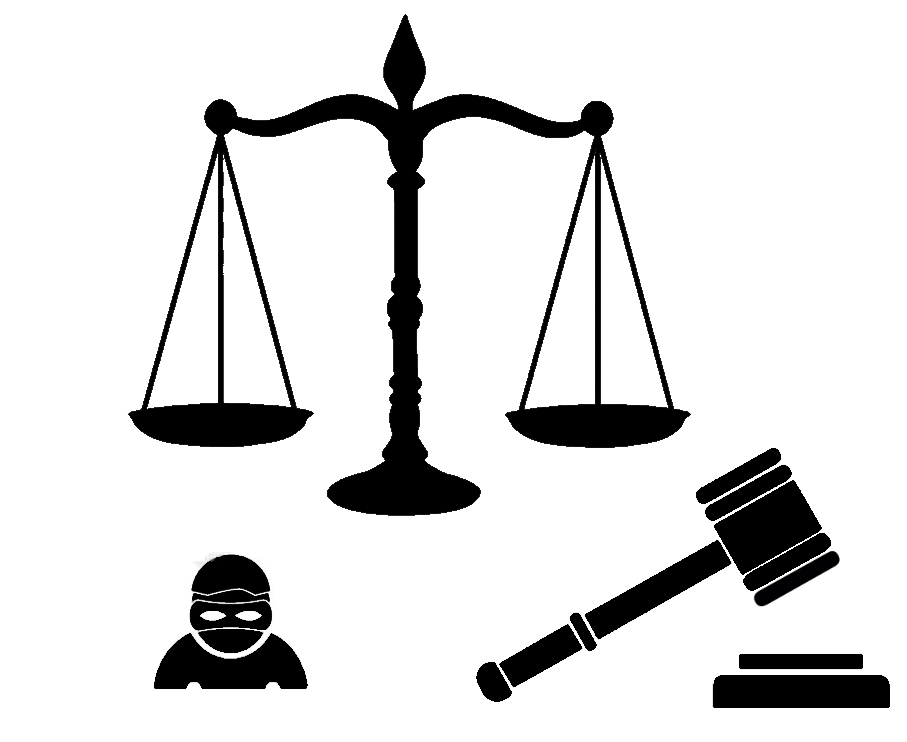
\includegraphics[width=14cm]{CaratulaIgnatenko.png}
  \vfill
  \vfill
  {\scshape\LARGE Modelos Líneales \par}
  \vspace{3cm}
  {\Large Ignacio Acosta - Sofía Itté - Mauro Loprete \par}
  {\Large 1er semestre 2021 \par}
\end{titlepage}
\tableofcontents
\setkeys{Gin}{width=0.8\textwidth}
\listoffigures
\newpage



\section{Introducción}
\begin{knitrout}
\definecolor{shadecolor}{rgb}{0.969, 0.969, 0.969}\color{fgcolor}
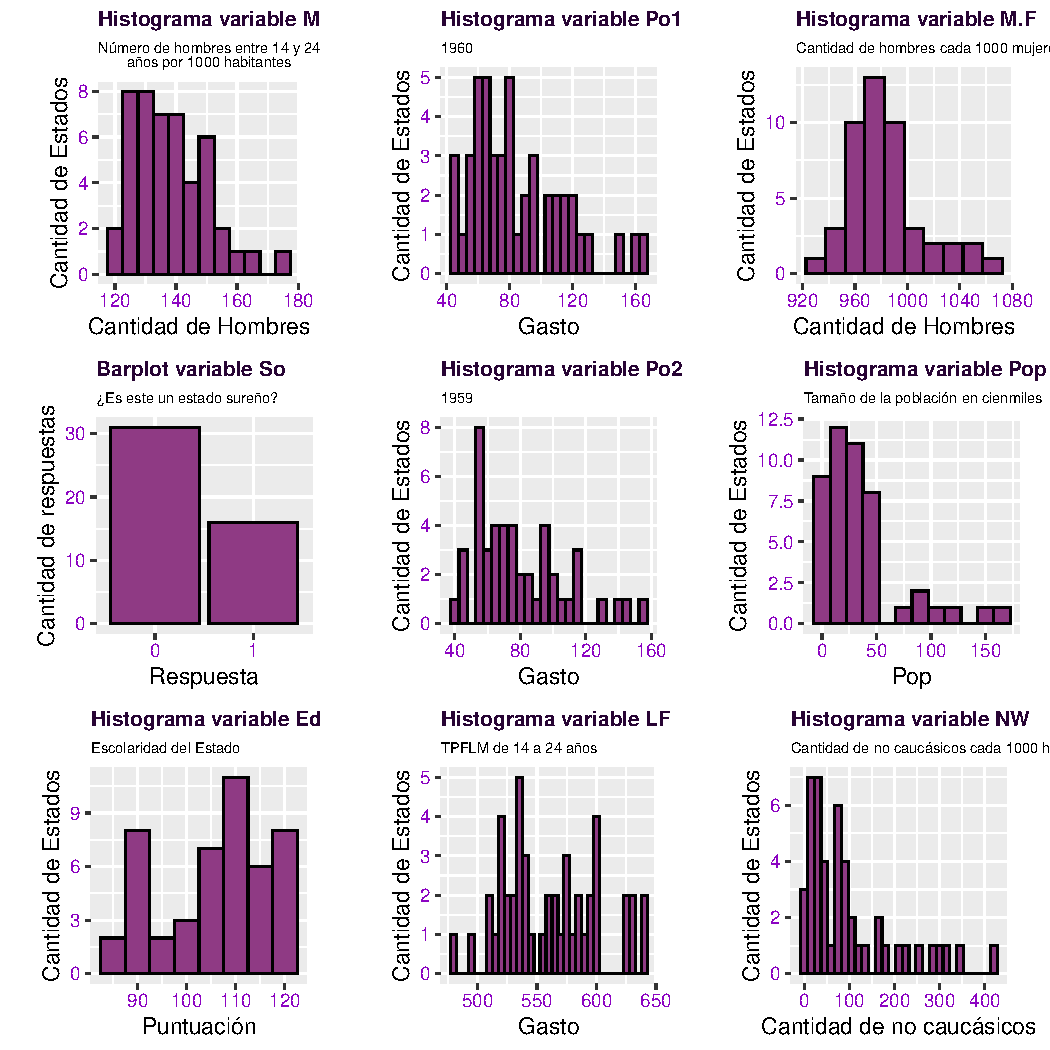
\includegraphics[width=\maxwidth]{figure/unnamed-chunk-2-1} 

\end{knitrout}
\newpage
\section{Análisis Exploratorio de datos}

El objetivo de esta sección es presentar las variables a estudiar y como las mismas se relacionan entre sí.
\\

Para ello se hará uso de distintas medidas de resumen univariadas y bivariadas, así como también un herramental gráfico variado que simplificará el entendimiento de las mismas.
\\

Es esta sección fundamental al momento de discutir el modelo final y como a partir de distintas técnicas estadísticas aprendidas en el curso se puede simplificar el \textit{modelo completo} que se presentará en la sección siguiente.

\subsection{Análisis Univariado}
En esta primer sección se hará especial enfásis en las variables por sí mismas.
\\

Se estudiarán medidas de resumen y a partir de histogramas tendremos un primer acercamiento a la distribución de las mismas y su comportamiento.

\begin{table}[h]
\begin{tabular}{|c|l|l|l|}
\hline
\textbf{Nombre} & \multicolumn{1}{c|}{\textbf{Descripción}}                                                                                                              & \multicolumn{1}{c|}{\textbf{Clasificación}} & \multicolumn{1}{c|}{\textbf{Unidad}} \\ \hline
\textbf{Y}      & Tasa de criminalidad, número de ofensas reportadas a la policía por habitante                                                                          & Cuantitativa                                &                                      \\ \hline
\textbf{M}      & Número de hombres entre 14 y 24 años cada 10000 habitantes                                                                                             & Cuantitativa                                &                                      \\ \hline
\textbf{So}     & Variables indicadora de los estados del sur (0=No, 1=Si)                                                                                               & Cualitativa                                 &                                      \\ \hline
\textbf{Ed}     & Indice que refeleja la escolaridad del estado                                                                                                          & Cuantitativa                                &                                      \\ \hline
\textbf{Po1}    & Gasto per cápita en policía realizado por el gobierno estatal o local en 1960                                                                          & Cuantitativa                                &                                      \\ \hline
\textbf{Po2}    & Gasto per cápita en policía realizado por el gobierno estatal o local en 1995                                                                          & Cuantitativa                                &                                      \\ \hline
\textbf{LF}     & \begin{tabular}[c]{@{}l@{}}Tasa de participación en la fuerza laboral civil de sexo masculino entre 14 y 24 \\ años, cada 1000 habitantes\end{tabular} & Cuantitativa                                &                                      \\ \hline
\textbf{M.F}    & Número de hombres por cada 1000 mujeres                                                                                                                & Cuantitativa                                &                                      \\ \hline
\textbf{Pop}    & Tamaño de la población del estado cada 100000 habitantes                                                                                               & Cuantitativa                                &                                      \\ \hline
\textbf{NW}     & Número de caucásicos cada 1000 habitantes                                                                                                              & Cuantitativa                                &                                      \\ \hline
\textbf{U1}     & Tasa de desempleo urbana de hombres entre 14 y 24 años cada 1000 habitantes                                                                            & Cuantitativa                                &                                      \\ \hline
\textbf{U2}     & Tasa de desempleo urbana de hombres entre 35 y 39 años cada 1000 habitantes                                                                            & Cuantitativa                                &                                      \\ \hline
\textbf{GDP}    & Producto bruto interno per cápita                                                                                                                      & Cuantitativa                                &                                      \\ \hline
\textbf{Ineq}   & Desigualdad del ingreso                                                                                                                                & Cuantitativa                                &                                      \\ \hline
\textbf{Prob}   & Probabilidad de encarcelamiento                                                                                                                        & Cuantitativa                                &                                      \\ \hline
\textbf{Time}   & Tiempo promedio de estadía en cárceles estatales                                                                                                       & Cuantitativa                                &                                      \\ \hline
\end{tabular}
\end{table}
\newpage
\subsubsection{Histogramas y Barplots}
\centering
\begin{knitrout}
\definecolor{shadecolor}{rgb}{0.969, 0.969, 0.969}\color{fgcolor}
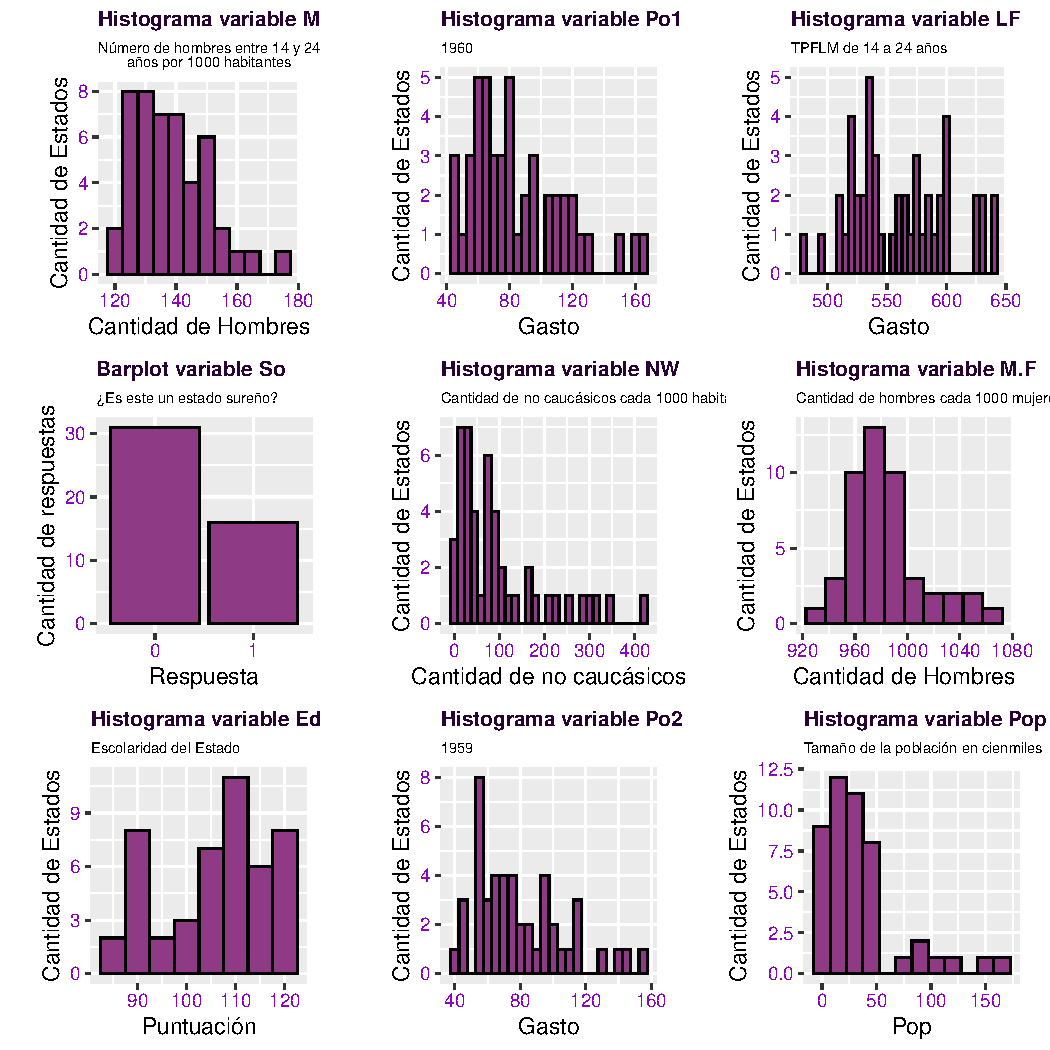
\includegraphics[width=\maxwidth]{figure/unnamed-chunk-3-1} 

\end{knitrout}
\newpage
\centering
\begin{knitrout}
\definecolor{shadecolor}{rgb}{0.969, 0.969, 0.969}\color{fgcolor}
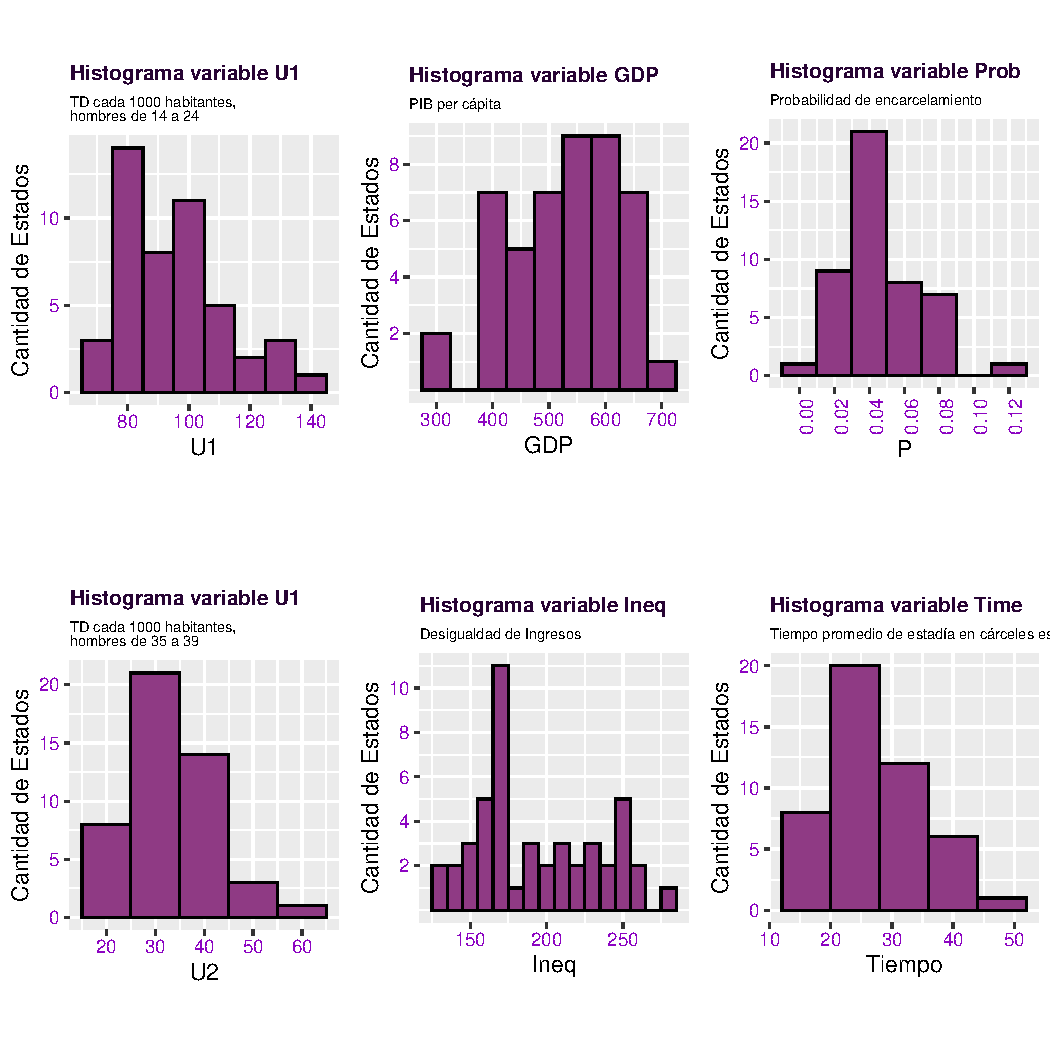
\includegraphics[width=\maxwidth]{figure/unnamed-chunk-4-1} 

\end{knitrout}
\newpage

\subsubsection{Correlación entre variables}

\begin{knitrout}
\definecolor{shadecolor}{rgb}{0.969, 0.969, 0.969}\color{fgcolor}
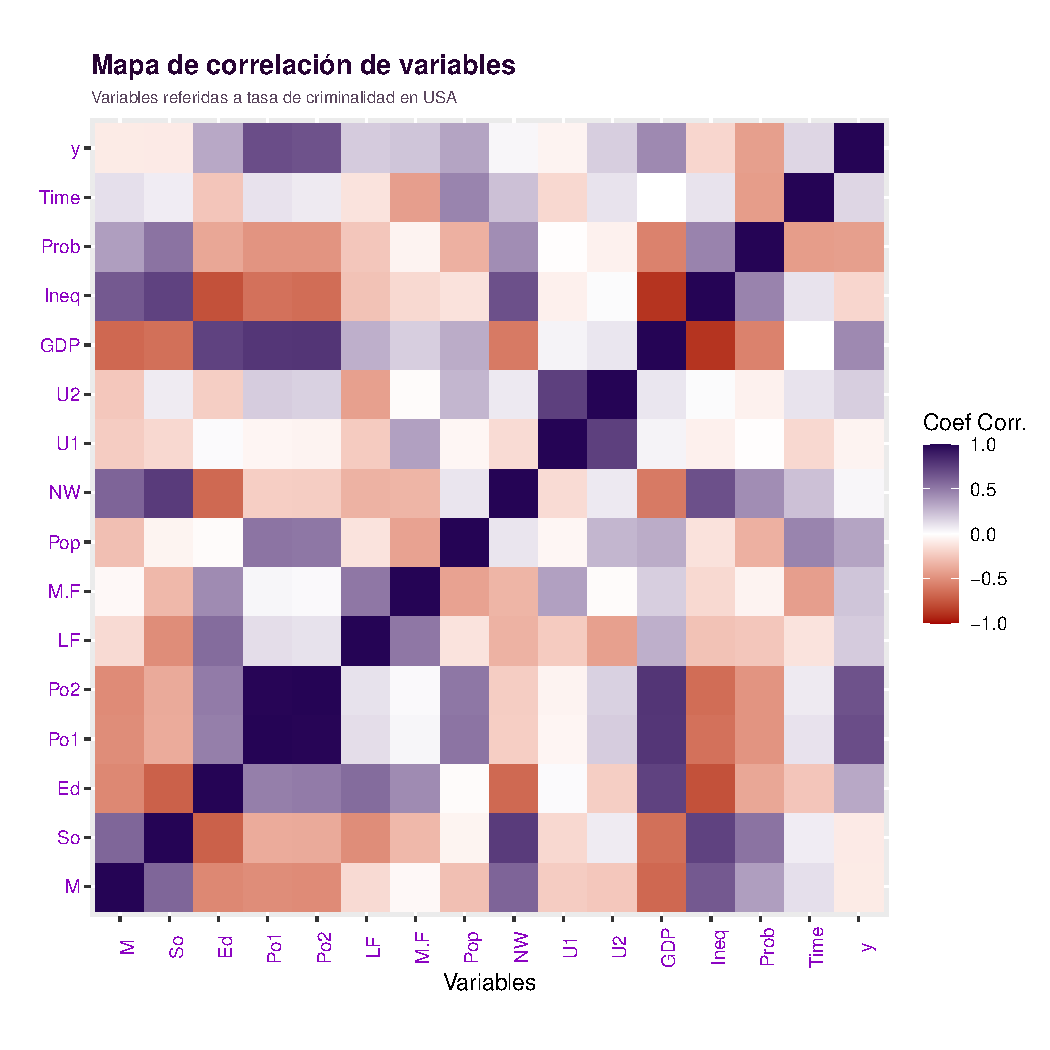
\includegraphics[width=\maxwidth]{figure/unnamed-chunk-5-1} 

\end{knitrout}
\end{document}
